\documentclass[a4paper]{article}

\usepackage[latin1]{inputenc}
\usepackage{palatino}
\usepackage{color}

\usepackage{hyperref}

\usepackage{chngpage}
\usepackage{graphicx}

\usepackage{booktabs}
\usepackage{multirow}



% nbuf command
\newcommand{\nbuf}{\textit{nbuf} }


%% a point to check
\definecolor{checkcolor}{rgb}{0.75, 0.75, 0.75}
\newsavebox{\definitionbox}
\newenvironment{checkit}{%
\begin{lrbox}{\definitionbox}
\begin{minipage}[t]{0.85\textwidth}%
}%
{\end{minipage}\end{lrbox}%
\begin{center}{\colorbox{checkcolor}{\usebox{\definitionbox}}}%
\end{center}}

\title{Automatic $n$-buffering for Big Data processing}
\author{Asbj\o rn Thegler}
\date{October 2015}

\begin{document}

\maketitle

\sloppy

\begin{abstract}
WRITE LAST

During the research, it was discovered that using three buffers was an arbitrary constraint, and
concluded that many use cases would benefit from a different number of buffers.
\end{abstract}

\newpage
\tableofcontents



\newpage
\section{Introduction}
It is hardly a secret that Big Data has become a huge topic over the last few years. Huge companies worldwide
compete on this new trend, and searching for 'big data trend' on Google reveals how popular this topic is, and is predicted to
be, for years to come. Forbes, CIO, ComputerWorld and Gartner all predict increases in the Big Data industry. (More)\\

There are many definitions to what Big Data really is. The truly new aspects of Big Data is to have large enough datasets to be able to find
and recognize patterns that previously were too vague or noisy to find, using only smaller datasets. When traditional data
processing techniques grow inapplicable, we must gain new knowledge to find methods to work with Big Data.

(Moore's Law for data growth? Harddisk space?)
Having data doesn't make any interesting results. The data must be processed, analyzed, and scrutinized. This is no small
task, and given that many new measurement tools generate tera-bytes of data per hour, back in 2013, we need to have mechanisms
in place for analyzing the data in a similar rate.\\


\subsection{Terminology}
(Should this be past tense?)
The first popularly known occurrences of the term 'Triple Buffering' stems from the computer graphics industry.
This is a technique where the graphics card renders images into 3 different buffers. Previous to this technique, a double buffer
was used. A 'front-buffer' and a 'back-buffer'. The renderer would render a frame into the back buffer, and the buffers would swap. Since no
synchronization exists between the renderer and the consumer, a buffer swap could happen in the middle of consumption,
resulting in what is known as 'screen tearing'. Some attempts at fixing this problem is know as 'vertical sync' or 'vSync'.
This included adding artificial delays to the renderer, to match the frame rate of the consuming screen.

To better solve this problem, a third buffer is employed, effectively making it 'Triple Buffering'. The renderer could now
switch between two back-buffers, and always have a free buffer to write a new frame to. If the consumer was too slow, frames
would simply be lost, with no greater loss to the viewer. This obviously require extra memory on the graphics card.\\


\subsection{Triple Buffering Big Data}
'Triple Buffering' within computer graphics is a different thing, though there are many similarities. We can translate some of the solution
to the field of Big Data. The bottlenecks of a graphics card are namely the rate of the renderer and the rate of the consumer. This translates to the IO problems we encounter when working with Big Data. The graphics industry solved the problem by utilizing more space, in the shape of an extra buffer
and in theory, this can solve, or at least mitigate, some of the IO problems related to Big Data.\\


The focus of this thesis project is to produce a framework or library that enables programmers to process or transform
large amounts of data in an efficient and concurrent way, without having to worry about concurrency issues and memory
management. The framework or library should be generic, such that it is as generally applicable as possible, while still
being useful and simple enough to understand for people who aren't familiar with multiprogramming. It is important to note
that this project in no way introduces new technology or uncovers scientific ground. This is a
study in working with existing technology to create a highly optimized and effective library.



\subsection{Motivation}
This project didn't manifest from thin air. Many people have probably seen it coming from a long
distance. Triple Buffering has been used many places, many times before, and it is a well-known
term. The reason why this project was started now, and not 10 years ago or in 10 years, is a combination and collision between
Moore's Law, data bus speed and the growing Open Source community, both within academia, but also within established industries.


\subsubsection{The IO Problem}
When processing data, it is relatively easy to increase the amount of computational resources, but moving
data to and from the computational resources results in IO, which quickly becomes a bottleneck. To process
data as fast as possible, we want to squeeze as much effect out of every available resource. When
processing data sequentially, the traditional method is to;

\begin{enumerate}
\item Load data into buffer from disk
\item Process or transform data
\item Write data back to disk
\item If there is more data; go to 1
\end{enumerate}

If the computational task of processing or transforming is large enough, the IO becomes negligible. If the
computational task is very small, most of the execution time will be spent waiting for IO. In the latter case,
there are two notable resources, which are being used in turn, namely the \textit{input stream} and the
\textit{output stream}. This means that only half of the resources are being used at any given moment. In this
case, we could have two concurrent workers, each swapping what resource they use, to utilize all of the resources
at any given time.

When the I/O becomes negligible, we have a very compute-heavy task. In this case, we can attempt to add more
compute resources, which in turn, will shorten the execution time. This means that we could have 5, 10 or 50
buffers, depending on how large the computation task is, in comparison to I/O.

(More?)


\subsubsection{The Generic Problem}
TODO: Rewrite to \textit{software bloat} Reading man pages is dreading

When programmers and developers write software, they are generally encouraged to utilize established
libraries as much as possible, instead of relying on their own ability to create elaborate and correct
code. Often, a programmer has to solve a specific problem, which can be translated into a general problem
which has already been solved multiple times. The productivity of the programmer can increase greatly,
when using tested and accomplished libraries. Some topics are inherently difficult for programmers, such
as memory management and concurrency, often leading to memory leaks and race conditions. When using
established libraries, these problems are often already addressed.

Within the Open Source community, it is common practice to make ones code available for others to use.
When multiple entities utilize the same code or library, bugs and race conditions are found, reported and corrected
much faster than when code is only used privately (link?). Over time, this often result in libraries that are
used globally, and has many contributors.

When a library does not exist for the specific problem, programmers must solve the problem themselves. This will
result in many programmers solving the same problem over and over again. At some point, someone will see the pattern
and pick up the task, and attempt to build a generally applicable library.

There are some pitfalls to using libraries to solve tasks. When a problem is simple, using a complex library might
be too much work, since many libraries has a ton of options that might be relevant. Reading the 'man'-page of any
Linux tool can be a daunting task, while often simple problems can be solved faster in other ways. Also, Open Source
projects tend to have organic growth. Without tight steering from some small group of committed developers, a project
will be monolithic and many people will classify it as 'bloatware'.

[cite Zawinski's law of software envelopment]
    Every program attempts to expand until it can read mail. Those programs which cannot so expand are replaced by ones which can.


\subsubsection{Use Cases}
The intended library can be used for several specific purposes. Many places, large amounts of data are being processed.
Following are a few use cases where using such a library is indeed a good solution.\\


Hash algorithms are designed to be compute-heavy. When hash-values are needed on very large local files, it would
be more efficient to use a n-buffering mechanism, and add buffers until the IO again becomes the bottleneck. The
command line tools md5sum and sha512sum both have implementations that read 512 bytes at a time, which results in
many IO operations, in case of large files, which could be avoided, if more memory is available for multiple buffers. Gathering statistics
on sensor data is also a brilliant use case.\\


When large amounts of sensor data are received via a network, they are usually written directly to disk, before
they get processed. In cases where much of the data is merely noise it could be good to have an option to process
the data the instant it arrives, instead of waiting until after is has been written to disk. This can include
gathering statistics, calculating hash values or filtering irrelevant data.\\\\

(More use cases?)



\subsubsection{Big Data and Complexity}
Complexity of algorithms doesn't matter with small data-sizes. Big Data makes complexity really important.

time to access disk compared to memory





\newpage
\section{Theory and Analysis}
This section will explain the ideas and thoughts that are used during the design and implementation of the framework.
The project has two main topics.

First there will be reasoning about concurrency and correctness. How to ensure that the
library will always terminate when used correctly.

Second, the project entails a lot of aspects related to data, IO and
how to handle the enormous amounts of data.

Finally, I will reason on what results I expect to get from this project, in relation to solving some of the problems touched upon in my motivation.



\subsection{Concurrency}
Concurrency has proven to be hard for the human mind to understand, design and work with. When done wrong, software can easily
include deadlocks or other race conditions. This section will explain some of the pitfalls of concurrency and how to avoid them.


\subsubsection{Flow and Deadlocks}
Concurrency done wrong can result in processes running out of control, or not running at all. The school-example used in teaching deadlocks to classes is known as the Dining Philosophers Problem, which was presented by E. W. Dijkstra in 1971. [Dijkstra, Hierarchical ordering of sequential processes]

Deadlocks and deadlock prevention is paramount when working with concurrency, but explaining why should be trivial at this point. I will suggest reading Concurrent Systems, by Jean Bacon [reference!], if you want to learn more on this topic. This project requires knowledge of how deadlocks can happen, and what measures can be deployed to avoid them, both theoretical and practical, but I will not explain further here.


\subsubsection{Finite-state Diagrams}
Any process can be interpreted as a finite-state machine. Doing so will help understanding the process, its possible states, and the triggers that will change the internal state of the process. This is known as the scientific body of "Automata Theory" and what I will elaborate on here, is a subset of this field.

To gain a better understanding of a finite-state machine, a finite-state diagram can be created. It is a tool that can be used to ensure that the process at hand reacts and interacts as expected. Finite-state diagrams are trivial to both create and understand, and can be used to reason about a process, as a development tool and as documentation about a certain system or process. It gives an abstract idea of how a concrete process progresses.\\

% State Diagram 1
\begin{figure}
	\begin{adjustwidth}{-0.5in}{-0.5in}
    \centering
    \def\svgwidth{\columnwidth}
    \input{figures/door.pdf_tex}
  	\caption{This is an example of a finite-state diagram. It represents a door which can be in 3 states, and there are 4 different transitions.}
	\label{figure:door}
	\end{adjustwidth}
\end{figure}

In figure \autoref{figure:door} there is an example finite state diagram. This diagram is quite simple, and shows how a door with a lock will behave.

There are 3 states, \textit{Open}, \textit{Closed} and \textit{Locked}. The process must be in either state at any one time. Further, there are 4 different events that can happen, \textit{open}, \textit{close}, \textit{lock} and \textit{unlock}. These can happen at any time, and the door will transition to another state. There are implicit transitions on every state, which lead to itself on events that there are not explicit transitions for. For example, locking an open door will make the door transition to the same state, while locking a closed door will make the door transition to the \textit{Locked}-state.\\

When explaining how the \nbuf framework works, I will use finite-state diagrams to show how the worker threads behaves. This helps understand how the threads are initialized, used and terminated, and more importantly, how they interact with each other through synchronization primitives.


\subsubsection{Synchronization Primitives}
Concurrent programming entails using some kind of multiprocessing. This is usually done by using multiple threads which can be scheduled individually on cores. This allows multiple thread to run simultaneous, using the same memory space. While sharing memory is very practical, it also brings several pitfalls that can seem in-obvious to a programmer who aren't used to concurrency. To solve these problems, it is necessary to use some kind of synchronization, to ensure \textit{thread-safety}.

All synchronization mechanisms are based on the hardware instruction \textit{test-and-set}. Using this instruction, locks, semaphores and queues can be implemented. These are all known as \textit{Synchronization Primitives}. These are abstractions, and are intended to make it easier to make more elaborate synchronization in systems. The primitives that are relevant to this project are the following:

\begin{itemize}
\item \textbf{Mutex} - A mutex is merely an advanced locking primitive. The name is derived from 'mutual exclusion'.
\item \textbf{Condition Variable} - A condition variable is a primitive that can be used to make threads wait for specific events.
\item \textbf{Future} - A future is a primitive that encapsulates the result of an asynchronous calculation for the calling thread. The naming is intended to be understood as; \textit{In the future I have this}.
\item \textbf{Promise} - A promise is a primitive that encapsulates the result of an asynchronous calculation for the executing thread. The naming is intended to be understood as; \textit{I will have to fulfil the promise}.
\end{itemize}


A \textbf{mutex} is basically a lock. It can be used to protect critical section of code. It is a higher-level construct, and automatically makes a thread wait, when it attempts to obtain the mutex while it is already taken.\\

A \textbf{Condition Variable} is a primitive which can be used to block threads on purpose. A thread can be set to wait on a specific condition variable, which means that it will block until another thread has notified one or all threads that are waiting on that specific condition variable. Most condition variables have a mechanism for notifying just one thread, or all threads. This is practical, since there might be cases where many threads are waiting, but only one can continue, and the other threads will have to wait for some time. In other cases, all threads might be able to continue working after this event. 

Normally, using a condition variable requires that some condition has to be true, before continuing, since many implementations allow threads to wake up spuriously, even though no threads has notified. In case of a spurious wakeup, the thread should be able to detect if the wakeup was due to a notification, or if it was spurious.\\

A \textbf{Future} is a primitive which is created by the calling thread, sometimes referred to as the master thread. This thread creates the future primitive and pairs it with a task that can be performed asynchronously. The task can be started, and the master thread can perform other calculations. When the master thread needs the result from the task, it can wait for the future to be finished, such that the result can be retrieved from the future.\\

A \textbf{Promise} is a primitive which is created by the calling thread, and passed off to another thread. From the promise, the calling thread can create a future. The worker thread which received the promise as a parameter can set the content of the promise when it exits, such that it can be retrieved.\\

When working with multiple threads, it is historically very hard to handle exceptions that happens in other threads than the master thread. When a thread encountered an exception, it would terminate, and throw away the exception. A solution was to define a shared exception variable prior to starting the task, which could then be used to inform about what happened to the thread. 

When using the Future-Promise constructs, exceptions are stored in the promise and re-thrown when the master thread attempts to retrieve the result through the future. This makes debugging concurrency a lot easier, since the exceptions are no longer thrown away, and doesn't require the programmer to declare exception variables before every asynchronous call.


\newpage
\subsection{Data Handling}
Working efficiently with data is no small task. There are many physical limits to what results we can obtain, but getting
to these limits often requires a lot of thought, since there are many abstraction layers between hardware and software. This section
will elaborate on how to work with these sizes of data in a correct and efficient manner.


\subsubsection{Optimal Buffer Size}
The size of a buffer

Buffer size should be less than the file size. If buffer sizes are 3*300M but file is 100M,
then it is inherently sequential.



\subsubsection{Data Marshalling}
When receiving and sending data to and from a stream, care should be taken to correctly de-serialize and serialize data.
(Google Proto-buffers)


\subsubsection{System Data Steams}
Why is output to disk fast, while input from disk is slow? Systems buffers.



\subsection{Theoretical Speedup with threads}
Using multiple threads will still only use one process. This can use all computational cores on a system, but will not be able to use other devices, such as extra CPUs or GPUs.



\subsection{Theoretical Speedup with devices}
Using multiple devices, such as GPUs can greatly affect the computational power. When performing the same task on many pieces
of data, one should always consider using a GPU, since it is massively parallel.






\newpage
\section{Design and Implementation}
This section will explain how the \nbuf framework has been designed and implemented. First I will identify and elaborate on the inherent requirements of such framework. Secondly, I will elaborate on the abstract idea of how the framework handles concurrency. Then I will elaborate on how the framework is to be used, and finally a technical description of how it has been built.


\subsection{Technical Requirements}
The \nbuf framework, being generic, should enable developers to create a wide array of software, which solves different problems. This can easily result in \textit{software bloat}, when software gets too much functionality. \nbuf should include features which is necessary to solve basic tasks, but a balance is important, when it comes to deciding what is necessary and what is not.

Follow are a list of functional and non-functional requirements which I deem important enough, to warrant further discussion:

\begin{itemize}
\item \textbf{Efficient and Parallel I/O} - The \nbuf framework must prioritize keeping the I/O resources busy as often as possible.
\item \textbf{Limited Space Guarantee} - When processing data, the framework must be able to keep a strict upper limit on allocated memory.
\item \textbf{Custom Processing} - The developer must have freedom in deciding how to process or transform the data.
\item \textbf{Input/Output Sensitivity} - The order of input and output must be identical, if the developer desires this.
\item \textbf{Output Selecting} - It must be possible to only output statistics, or only output transformed data.
\item \textbf{Output Filtering} - It must be possible to only output parts of the transformed data.
\item \textbf{Guaranteed Termination} - The framework must terminate if and only if it works with a finite amount of data.
\end{itemize}

These features are all items that are important, if this framework should be generally applicable to most sorts of projects working with any kind of I/O. In the next few sections, I will explain what these requirements entail, and how they have been solved.

\subsubsection{Efficient and Parallel I/O}
The entire project attempts to maximize the use of the available I/O resources on a system, when processing incoming data. If there are solutions which allows for a larger rate of processing data, then the \nbuf framework does not perform as it should. This is a primary goal, and should at all times be respected. This non-functional requirement will only be observable when running the system.

To achieve this goal, it is necessary to use some kind of concurrent programming methods. It is impossible to keep all system I/O resources busy, using only a single processing thread, since there will often be at least two resources, and there will be real processing work to be done as well. 

As mentioned earlier, this has been done multiple times with a triple buffer system, where three processing threads would perform all three tasks in parallel. One thread would keep the input resource busy, would thread would keep the output resource busy, and one thread would perform the processing work.\\\\
 

In a new framework, we can evaluate and rethink this triple-buffer-idea. In cases where there are is a high amount of processing work, a triple buffer system will be waiting for the thread performing the real work. On a single core system, this is not a solvable problem, since we can't speed up the execution speed. A good computer scientist might be able to optimize the program, but this has a limited usefulness. 

On the other hand, if we have a system with multiple execution cores, it would be possible, and a very good idea too, to utilize the extra computational powers to speed up the execution time. This requires that the work can be done in parallel, which is not always the case. In cases where the work can be parallelized, the extra processing can be utilized, until the rate at which data can be processed matches the lowest rate at which data can be read or written. This will, in turn, maximise the use of the available I/O resources on the system.

The framework must be able to use multiple processing cores, and support the developers in performing parallel work.


\subsubsection{Limited Space Guarantee}
The main memory available on a computer system is rarely a hard limit. Usually, when a process starts allocating more main memory that are available, some data is moved to a swap-partition on the systems disk drive. This results in very high delays when allocating more memory, and trying to read data which has been moved to the swap-partition. When trying to work efficiently, this is a killer, and any processes doing this, will completely stall the entire system. 

For this reason, it is important to be aware of the memory usage of all processes on a system. Software which greedily allocates huge amounts of memory, or simply forgets to deallocate memory (resulting in memory leaks) is to be considered buggy, and will not be used in critical systems. It is a minimum requirement for all software to deallocate memory, and many programming languages employs different methods such as garbage-collectors or scoped variables to ensure that memory is deallocated when it is no longer used.\\\\


Back in the 1994, Bjarne Stroustrup [The Design and Evolution of C++] introduced the term and programming idiom \textit{RAII}, short for \textit{Resource Acquisition Is Initialization}. This has become a widely used technique which gives several advantages. In RAII all memory required for an object to exist, or a process to run, will be allocated during initialization. This gives the advantage of ensuring that the process will not slowly allocate additional memory, and over time exhaust the main memory resources.

The \nbuf framework will require memory and as such, it should be possible to give an upper limit on how much memory it will consume. If the process consumes more memory than it has been given, then there is a risk that the system will start using the swap-partition, which is bad. The given upper limit should be respected at all times.


\subsubsection{Custom Processing}
The developer using the \nbuf framework will only use it, if it gives the freedom to solve whatever task he desires. Some cases warrant only gathering statistics about the data at hand, others require a slight transformation or reorganisation of data. These cases should be solvable using the framework. 

The worker performing the real processing must be programmable by the developer. When the worker has a buffer full of data, it must be up to the developer to decide how to process the buffer. There should be allocated some memory for gathering statistics, and it should be possible to alter the data in the buffer. What the developer intends to do with the data in the buffer is to no concern of the framework, but the framework should support the intentions of the developer.\\\\

Here are the three identified types of data that the developer might want to extract and save when processing data:
\begin{itemize}
\item \textbf{Input-wide Accumulated Data} - This data is to be accumulated across the entire input data.
\item \textbf{Buffer-wide Accumulated Data} - This data is to be accumulated across one buffer, or any smaller amount of data.
\item \textbf{Transformed Data} - This data is an in-memory transformation of the data in the buffer.
\end{itemize}

These three types of data must be creatable and extractable, when using the framework.


\subsubsection{Input/Output Sensitivity}
The case where we want to find the minimum value, the maximum value and the average value in a file is a very simple example. It is of linear complexity and simply requires a single run through, in no specific order. This is a highly parallelizable algorithm and is a brilliant example case for this kind of framework. 

Another case, creating an md5-sum for example, requires that the data will always be parsed in the same order, every time. For simplicity and practicality, it has been decided that the sum must be calculated chronologically, meaning that the first data in the file must be hashed first. This is an algorithm which cannot easily be parallelized to any extend, however, it does heavily rely on I/O, and would benefit from using a framework such as \nbuf.\\\\

To accustom to this need, it must be possible to decide that the framework should always parse the data in-order and not parallelize the calculations. This can, of course result in not gaining a maximum utilization of the I/O resources, but this is always the choice of the developer and a requirement at hand, related to the task. 


\subsubsection{Output Selecting}
When calculating the md5-sum of a file from disk, there is no need to write the content of the file back to disk. In this case, it must be possible to not occupy the output resource with needless work. If the framework occupies resources it does not need, it can lead to other processes waiting for the resources which will result in a slower system. Therefore, it should be possible to decide what parts of the data that should be retrievable from the framework.


\subsubsection{Output Filtering}
In cases where parts of the data might not be interesting, or the transformed data is smaller than the original data, it would be ideal to filter data such that it does not occupy more memory than necessary. This is indeed relevant in the use case where the developer receives data from sensors, which in periods doesn't measure interesting data. This could be a rain gauge, which reports 0 millimetres for many months a year.


\subsubsection{Guaranteed Termination}
The framework must terminate when it works with a finite amount of data. The framework can never be fool-proof, but it should always terminate when it receives an indication that there are no more data, often an EOF. If the developer employs an infinite loop when processing data, this promise cannot be kept, but the framework should never result in a deadlock or a spinlock.\\\\\\


These are the technical requirements that I have decided that the \nbuf framework will have to live up to, to be generally useful. During the remainder of this section, I will discuss what actions I have taken to ensure that these requirements are fulfilled.



\newpage
\subsection{Abstract Overview}
When performing concurrent programming, it is custom to have a master thread which prepares all the communication channels, the worker threads and allocates all the resources required to perform the concurrent work. This is part of the RAII idiom, and will be a central part of the design of the system. In this section I will give an abstract overview of how the master thread will prepare the environment to enable the worker threads to run, and how the workers synchronize with each other, to ensure correctness and to avoid race conditions.


\subsubsection{The \nbuf master}
The initialization of the \nbuf framework entails a few tasks:

\begin{itemize}
\item Sanity checking settings
\item Allocating system resources
\item Initialize worker synchronization mechanisms
\end{itemize} 

After parsing the data, the master thread will be responsible for:

\begin{itemize}
\item Deallocating system resources
\item Termination of worker threads
\item Returning the required data
\end{itemize} 

While allocating system resources should be a job for the master thread, due to RAII, I will deviate slightly when it comes to allocating the worker buffers. Sharing memory between threads require careful coordination. This is part of why concurrent programming is inherently hard. If I can establish a method where less memory sharing is used, it will make the framework less complex, easier to understand and more maintainable. For this reason, some allocation will be left to the worker threads. This will include the worker buffers and the memory for the buffer-wide accumulated data, which are the largest part of the required memory.



\subsubsection{The \nbuf workers}

Each worker has its own buffer which it will use for reading into, processing and writing from. This buffer is not shared with any other worker.\\

In \autoref{figure:state-diagram} is a finite-state diagram which shows how each worker in the system transfers from state to state, and in \autoref{table:transition} the related transition table can be seen. It is important to note that there are two \textit{critical} states. These states are intended to mimic the importance of a critical section, as known from concurrent programming\\\\

% State Diagram 1
\begin{figure}
	\begin{adjustwidth}{-0.5in}{-0.5in}
    \centering
    \def\svgwidth{\columnwidth}
    \input{figures/state1.pdf_tex}
  	\caption{\nbuf worker state diagram. This finite-state diagram shows how the workers can change states, based on events. Further explanation on how the transitions happens can be found in the related transition table which can be seen in \autoref{table:transition}.}
	\label{figure:state-diagram}
	\end{adjustwidth}
\end{figure}


% NBUF Worker State Transition Table
\begin{table}[]
\begin{adjustwidth}{-0.5in}{-0.5in}
\centering
\begin{tabular}{@{}llll@{}}
\toprule
\textbf{Current State}         & \textbf{Input}           & \textbf{Next State} & \textbf{Result}                                                                                                      \\ \midrule
Initialization                 & \textit{ready}           & Read Wait           & \begin{tabular}[c]{@{}l@{}}Worker is ready for reading, but has \\ to wait for the read-resource.\end{tabular}       \\ \midrule
Read Wait                      & \textit{read available}  & Read Critical       & \begin{tabular}[c]{@{}l@{}}Worker can now read, which blocks \\ other workers from this state.\end{tabular}          \\ \midrule
\multirow{2}{*}{Read Critical} & \textit{data read}       & Execute             & \begin{tabular}[c]{@{}l@{}}Worker read some data, and can now \\ process it.\end{tabular}                            \\ \cmidrule(l){2-4} 
                               & \textit{nothing read}    & Exit                & \begin{tabular}[c]{@{}l@{}}Worker read nothing, and the work is \\ finished.\end{tabular}                            \\ \midrule
Execute                        & \textit{done execute}    & Write Wait          & \begin{tabular}[c]{@{}l@{}}Worker has processed its data, but has \\ to wait for the write-resource.\end{tabular}    \\ \midrule
Write Wait                     & \textit{write available} & Write Critical       & \begin{tabular}[c]{@{}l@{}}Worker can now write, which blocks \\ other workers from this state.\end{tabular}         \\ \midrule
Write Critical                  & \textit{done write}      & Read Wait           & \begin{tabular}[c]{@{}l@{}}Worker is ready for reading again, but \\ has to wait for the read-resource.\end{tabular} \\ \midrule
Exit                           & \textit{}                &                     & No transition exists from the exit state.                                                                            \\ \bottomrule
\end{tabular}
\caption{\nbuf worker state transition table. This table shows the states, acceptable input and transitions within the \nbuf worker state diagram, which can be seen in \autoref{figure:state-diagram}.}
\label{table:transition}
\end{adjustwidth}
\end{table}


To clarify the intention behind how the workers interact, I will here explain how a worker move through the states in the diagram. Remember that there are a finite amount of workers, and that the input resource will be empty, at some point. In cases where the input will never empty, we will not expect the program to terminate.

First, all workers begins in the \textit{Initialization}-state and, it will move into the "Read Wait"-state. When the single read resource is available, a worker will move into the \textit{Read Critical}-state. This state is exclusive, since only one worker can read at a time. This may be any of the workers which are in the \textit{Initialization}-state.

We now follow the worker in the \textit{Read Critical}-state. At this point, two things can happen. Either, the worker receives data from the resource, or it does not receive data. If it does not receive data, it will be because there is nothing to receive from the input-resource. If it receives data, the amount of data it receives does not matter, the buffer may be almost empty, or it may be full. 

With data in the buffer, the worker will move to the \textit{Execute}-state, and another worker can enter the \textit{Read Critical}-state. Note that the \textit{Execute}-state is not exclusive, and that multiple workers can perform this step in parallel. 

Now, the worker will process the data located in the buffer, and produce whatever data the developer has decided. When the worker has finished processing, it will move into the \textit{Write Wait}-state. In this state, the worker will wait for the single output resource to become available. When it becomes available, the worker will move to the \textit{Write Critical}-state and occupy the output resource. When the worker has written the content of its buffer to the output-resource, it moves to the \textit{Read Wait}-state, since it has finished the cycle, and can read new data into the buffer. 

At some point, the read resource has no more data, and the worker will not receive data during the \textit{Read Critical}-state. At this point, it will move to the \textit{Exit}-state, and stay there until thread termination, which will be initiated by the master thread.\\\\

% State Diagram 2
\begin{figure}
	\begin{adjustwidth}{-0.5in}{-0.5in}
    \centering
    \def\svgwidth{\columnwidth}
    \input{figures/state2.pdf_tex}
  	\caption{\nbuf worker state diagram with a queue. This is an evolution from \autoref{figure:state-diagram}. The workers cannot overtake each other when they are inside the queue.}
	\label{figure:state-diagram-queue}
	\end{adjustwidth}
\end{figure}

It is clear that this state diagram will serve the general purpose, but \textbf{Input/Output Sensitivity}-requirement can not be supported this way. To comply with this requirement, the framework must support utilizing an altered state diagram which can be seen in \autoref{figure:state-diagram-queue}. In this diagram a FIFO-type queue has been added. This means that the worker thread that entered the queue first will reach every new state before every other thread. Further, a \textit{Execute Wait}-state has been introduced along with introducing an \textit{Execute Critical}-state, which replaces the original state.\\\\



\autoref{figure:state-diagram} and \autoref{figure:state-diagram-queue} are two extremes. One entails full parallelization, the other is inherent sequential. There are two middle-way solutions. 

% State Diagram 3
\begin{figure}
	\begin{adjustwidth}{-0.5in}{-0.5in}
    \centering
    \def\svgwidth{\columnwidth}
    \input{figures/state3.pdf_tex}
  	\caption{\nbuf worker state diagram with a smaller queue. This is an evolution from \autoref{figure:state-diagram-queue}. The workers cannot overtake each other when they are inside the queue, but the execution step can be performed and finished in parallel. This means that workers entering the queue at the \textit{Read Critical}-state has to go to the \textit{Write Critical}-state in the same order.}
	\label{figure:state-diagram-semi-queue}
	\end{adjustwidth}
\end{figure}

If we want the output to be sequential, but the execute step to be performed in parallel we will have to introduce a different kind of queue. This queue will merely ensure that the order of threads entering the \textit{Write Critical}-state matches the order they arrived at the \textit{Read Critical}-state. This will still allow parallel processing, but threads will not be able to overtake each other in the cycle, outside of the \textit{Read Wait}-state. The third alternative can be seen in \autoref{figure:state-diagram-semi-queue}.

% State Diagram 4
\begin{figure}
	\begin{adjustwidth}{-0.5in}{-0.5in}
    \centering
    \def\svgwidth{\columnwidth}
    \input{figures/state4.pdf_tex}
  	\caption{\nbuf worker state diagram with a smaller queue. This is an evolution from \autoref{figure:state-diagram-queue}. The workers cannot overtake each other when they are inside the queue, but the write step can be performed and finished in parallel.}
	\label{figure:state-diagram-shared-accumulator}
	\end{adjustwidth}
\end{figure}

The other middle-way solution can be seen in \autoref{figure:state-diagram-shared-accumulator}. This entails having a sequential execute-step, but the order of the output does not matter. In this setup, the threads will have to arrive in the \textit{Execute Critical}-state in the same order they were in the \textit{Read Critical}-state.\\\\

Considering these four configurations, we can reason about how they relate. In \autoref{table:state-relation}, it is clear that they must all exist, due to combinations of different requirements.\\\\

\begin{table}[]
\begin{adjustwidth}{-0.5in}{-0.5in}
\centering
\begin{tabular}{@{}lll@{}}
\toprule
\textbf{Finite-State Diagram}                     & \textbf{Sequential Execution} & \textbf{Input/Output Sensitivity} \\ \midrule
\autoref{figure:state-diagram}                    & No                            & No                                \\ \midrule
\autoref{figure:state-diagram-queue}              & Yes                           & Yes                               \\ \midrule
\autoref{figure:state-diagram-semi-queue}         & No                            & Yes                               \\ \midrule
\autoref{figure:state-diagram-shared-accumulator} & Yes                           & No                                \\ \bottomrule
\end{tabular}
\caption{Configurations of the requirements, related to the finite-state diagrams. The figures have all been explained in-depth previously.}
\label{table:state-relation}
\end{adjustwidth}
\end{table}


But, there are even more possible configurations. There are cases where we want to ignore the \textit{Write Wait}-state and the \textit{Write Critical}-state, since the \textbf{Output Selecting}-requirement requires that we can turn off outputting the content of the buffers. This voids some of the configurations, but for simplicity, we will still consider these four configurations, and merely perceive that the work to be done in these two steps is non-existent.\\\\

This concludes the requirements to the the \nbuf framework. A framework which supports all of these items, should be generic enough to be useful, while still being practical.


\subsection{Algorithmic Overview}



\newpage
\subsection{Framework Interface}
When building a framework for other people to use, it is important to keep a clean, intuitive and usable interface. While man-pages are very useful, they can be dreading to read, for the non-guru. There are several ways to design a clean interface. Some developers tend to require a ton of configuration to do the simplest of things \footnote{The linux-command \textit{find} is a good example of non-intuitive CLI. You would expect the first argument to be the filename you want to find, but you need to specify the filename with -name.}, while others merely have sane defaults, and requires configuration to use the more advanced features\footnote{The linux-command \textit{locate} does what you would expect, it locates files with the name you supply as the first argument.}.\\

First, I need to identify what input is required to configure the \nbuf framework. Here is a list of input, along with example defaults:
\begin{itemize}
\item \textbf{Input Stream} - The framework can default to read from \textit{stdin} \footnote{Standard input is a standard stream used on most *NIX systems, along with standard error and standard out. They are known as \textit{stdin}, \textit{stderr} and \textit{stdout}.}.
\item \textbf{Processing Method} - The framework can default to doing nothing with the input data.
\item \textbf{Sequential Execution} - This is a bool, and the framework can default to performing parallel execution.
\item \textbf{Output Stream Enabler} - This is a bool, and can default to true.
\item \textbf{Output Stream} - In cases where output from the worker buffers is desired, this must can be supplied. It can also default to \textit{stdout}.
\item \textbf{Output Filter Enabler} - This is a bool, and can default to false.
\item \textbf{Output Filter Method} - In cases where the output should be filtered, a filtering method must be supplied. It can default to terminate the program, since not filtering would signify a user error.
\item \textbf{Number of Threads} - The framework can default to an arbitrary number, e.g. 3 threads.
\item \textbf{Memory Limit} - The framework can default to an arbitrary number, e.g. 100 megabyte, which most systems should have readily available.
\item \textbf{Data Chunk Size} - The amount of data that should be processed at once, by the processing method. This can default to the amount of data given per thread.
\item \textbf{Input/Output Sensitivity} - This is a bool, and can default to false.
\end{itemize}

This is the configuration that the framework must accept. They are, however, different types, and as such, they should be handled differently. Two of the input parameters are code references. There are several ways to insert code to be executed into programs. Many languages support method-overwriting, when working with objects. This could entail subclassing an object, when a developer requires to use the system. 



\subsection{Multithreading with \textit{std::thread}}
The \nbuf framework has been built using C++11. A new feature in C++11 is the support for native multithreading, and not depend on external libraries to execute parallel threads. Before C++11, it was necessary to call the POSIX thread library\footnote{The POSIX thread library is also known as pthreads.} directly, which did not offer many abstraction layers. 

The new thread library included in C++11 is referred to as std::thread. This library uses POSIX threads, but implements a much nicer abstraction layer, which allows the developer to ignore certain aspects. This allows for higher productivity and less complex code. This, in turn, makes the code easier to maintain.\\

When the \nbuf framework is started, the master thread will create \textit{futures} matching the number of worker threads. The master thread will expect each future to contain a pointer to the accumulated data from a single worker thread. Each worker thread will be initialized with a promise, which they are expected to fulfil. When they have reached the \textit{Exit}-state, they return the accumulated data to the promise, and the master thread will gather all results. The results will be combined, and this will be the result returned from the framework. A combined, accumulated set of data.\\

The framework has been designed to require as little synchronization as possible. While this has decreased the complexity of the framework, it has not completely eliminated the need for synchronization. The default case, without \textit{Input/Output Sensitivity} and without \textit{Sequential Execution} requires only two mutexes, which will never be locked at the same time. These two mutexes will manage each of the critical sections, related to the I/O resources. \\

When a critical section is required near the execution-step, it will also require a mutex. In this case, more synchronization is necessary, since the workers will also have to keep stay in the same order, at some point (all but the first configuration in \autoref{table:state-relation}. A worker-queue must be implemented, to ensure that threads are kept in order. There is no native synchronization mechanism for this kind of problem, but one can be built using \textit{condition variables}.\\

[ details on how to build a thread-queue ]\\

These are the technical details, related to how the \nbuf framework handles concurrency with the \textit{std::thread}-library.


\subsection{Multiprocessing with OpenCL}
[ details on how to work with OpenCL, even though this has not been built into the framework, it can still be utilized in the workers, since they can call OpenCL individually. ]\\


\subsection{Current Limitations}
[No queue, but supports sequential execution. This can, however, risk not being in order.]
[Either filter or full output, not both]

\newpage
\section{Experimentation and Benchmarking}
The \nbuf framework has two primary goals. It has to be efficient, and it has to be usable. The first goal can be measured quantitatively, the second cannot. This section will focus on deciding how efficiently this framework can work with system I/O. 


\subsection{Experimental Setup}
The framework solves a practical problem, namely it tries to fully utilize the speed of disks, bandwidth of networks, etc., and therefore it must be benchmarked in a practical environment to prove its effectiveness. This however, will add a lot of uncontrollable factors, to the results of the benchmarking. This section will elaborate on how different factors can affect the benchmarking, and how to eliminate these factors.\\

What I would like to measure is \textit{throughput}. The throughput can be measured as bytes processed per second. This clearly depends on how much execution work is required, and how much computational resources are available. If enough computing power is available though, the throughput depends less on the computation task.\\

I have decided that the benchmarking calculation is as simple as a search for minimum and maximum and calculating an average value. The naive implementation is simply a sequential loop which sums the values, while looking for minimum and maximum values and counting the amount of values. This implementation can be used as a baseline to test how much faster the \nbuf framework can perform these calculations. If the framework is slower than this naive implementation, then the framework is useless.\\

The benchmarking will be done on a machine with a Intel Core i7-2600K CPU 3.40GHz x 8. This is a processor with 4 cores, all with hyperthreading. On a system, it will appear to have 8 logical cores, but it can only run 4 hardware threads at a time. Futher, the system has 4 * 4GB of DDR3 1333MHz as main memory. This will sum up to 16 GB of main memory. Finally, the machines has a Samsung 500GB hard disk drive, with 16MB cache and 7200 RPM. The machine runs Ubuntu 14.04 64-bit as operating system. 


\subsubsection{From disk}
In many cases, the framework will have to work with a stream of data from a disk drive of some sort. In this case, the maximum throughput is limited by the rate at which we can read data from the disk, and write back to disk. Here we have to keep two things in mind, when experimenting.\\

First, most operating systems keep a cached version of files in memory, as long as the memory isn't used for anything else. This has been a mystery to many new Linux-users, and has sprouted many helping words\footnote{http://linuxatemyram.com explains very nicely how Linux caches files when there is available main memory.}. This easily results in wrong experimental results, when benchmarking throughput from disk.

Imagine performing an experiment twice, which includes timing how fast a file is read from disk. The first run will fetch the file from disk, and the experiment will return expected results. When starting the second run, there is a good chance the file is still in memory, and the operating system will therefore not fetch the file from disk, but merely return the cached version. This will result in a much faster benchmark for the second run, for the wrong reasons.

Second, the operating systems doesn't write your file to disk, just because you tell it to. It has to schedule all disk I/O and therefore it keep an internal buffer of data to be written to disk. This means that when some code writes to a file-stream, it will return before the data is actually written to the disk. The data is copied to another part of the system memory, and kept there until the OS decides to write it. The size of this buffer can vary, depending on how much memory the OS keeps to itself. When the buffer is full, the OS is forced to wait to disk, and let the program wait, until the OS has enough memory to copy the data from the program. To show how large the wait on disk input and disk output is, a simple experiment has been conducted.\\

The I/O experiment is meant to show the different between return times when performing disk input and disk output, when the operating systems manages the I/O. First, a file with 1GB of data is located on a file, on a consumer-grade hard disk drive. The OS file cache is emptied, a timer is started, and the program starts reading the entire file into main memory. When returning from the read, the timer is stopped and the resulting time duration is printed. Then a timer starts, and the program starts writing the 1GB data to a new file on the disk drive. When the OS returns to the user-code, the timer is stopped and the duration is printed. The experiment is repeated 20 times, after letting the operating system flush the buffer to disk, to ensure consistent results. The results can be seen in \autoref{table:io-test}.\\

\begin{table}[]
\begin{adjustwidth}{-0.5in}{-0.5in}
\centering
\begin{tabular}{@{}lll@{}}
\toprule
\textbf{Action}                & \textbf{Average time taken}               & \textbf{Standard Deviation / Average} \\ \midrule
Reading 1GB of data from disk  & 13411522 $\mu s$                          & 0.0281                                \\ \midrule
Writing 1GB of data to disk    & 541844   $\mu s$                          & 0.0128                                \\ \midrule
Copying 1GB in memory          & 184583   $\mu s$                          & 0.0046                                \\ \midrule
Processing 1GB in memory       & 4757252  $\mu s$                          & 0.0068                                \\ \bottomrule
\end{tabular}
\caption{The results from the disk I/O experiment on the actual hardware. Note that when writing data to disk, the operating system performs \textit{latency hiding}, which is why we observe much faster \textit{writing} that \textit{reading}. These are the timings we should expect to see when reading or writing 1GB of data to disk.}
\label{table:io-test}
\end{adjustwidth}
\end{table}


When this has been concluded, we know that the throughput of the \nbuf framework, is limited by the rate at which it can read data from the disk. The throughput of the framework should be as close to this as possible, to exhibit efficient I/O. If the framework can parse data faster than the disk loading times, it is a clear warning that something doesn't work as expected.


\subsubsection{From memory}
In comparison, main memory on a system suffers from much lower latency, than disk. This means that the potential throughput is much larger, when processing data that are already in memory. The experiment conducted here, merely copies 1GB of ram from one allocation to another. It is not necessary to test reads and writes, since they are essentially the same, in memory.\\

The results in \autoref{table:io-test} clearly shows that working with data that is already in-memory is much faster than when it has to be fetched from disk, to no surprise. Also, the timings are much more consistent, since we aren't working with a spinning metal disk that has to seek and find.\\

We can use these results to gain a higher confidence, when benchmarking the \nbuf framework. When testing the framework with a disk file-stream, the results are subject to these long load times. If we pre-load data to memory, it means that we can actually benchmark the framework to its limit, be it due to software or hardware, instead of merely testing the loading times from disk.


\subsection{Experimental Results}
Every experiment has been run 20 times, averaging the results and calculating the standard deviation. In the experiments where data is read from disk, the file cache has been cleared just prior to starting the experiment. Further, all non-critical software running on the experiment machine was terminated, to ensure that there was as few other processes running on the system. While this was possible to a large extend, it is still necessary to keep in mind that this is a live and running Linux system, so some inconsistency between experimental results are to be expected.


\subsubsection{From disk}
The results from running the experiment with parallel execution can be seen in \autoref{figure:disk-par}, and with sequential execution in \autoref{figure:disk-seq}. The practical timings from \autoref{table:io-test} tell us that the rate at which we can read 1GB data from the hard disk on the actual system is approximately 13.4 seconds. Further, the processing takes approximately 4.8 seconds. Performed sequentially, we can add the timings, this becomes 18.2 seconds.\\

The best result we get is approximately 15.1 seconds, which was achieved with 2 threads and using 1GB of memory. The result is quite close to the practical limit of 13.4 seconds. It is worth noticing that the system performs much worse when using more than 8 threads. This is probably due to many unnecessary context-switches, since we can only schedule up to 8 threads on the system.\\

It it difficult to say why the system performs so much worse with less available memory. The smaller amounts of memory will result in less memory allocated per thread, and in turn result in many smaller I/O operations. However, the experiments with 10M available memory performed even worse than the 1M experiments. I am unable to explain why.\\

The key points are to let the framework have as much memory as possible, and not running more threads than there are hardware support for. 

% Disk Parallel
\begin{figure}
	\begin{adjustwidth}{-0.5in}{-0.5in}
    \centering
     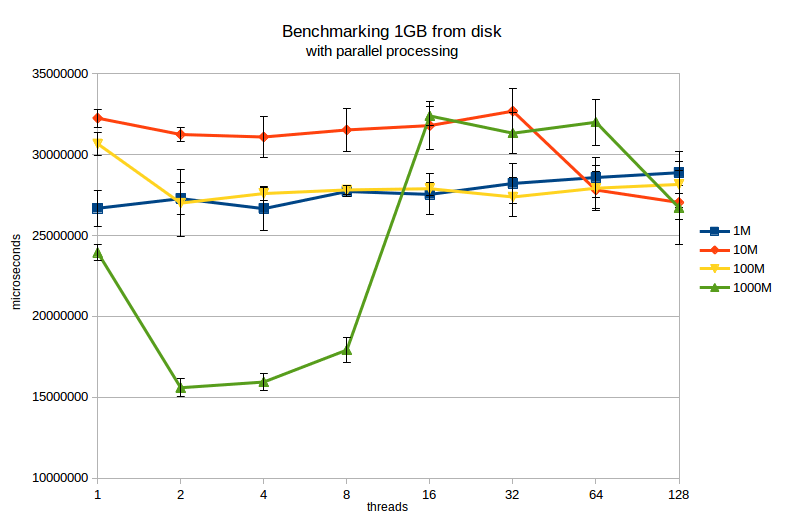
\includegraphics[scale=0.7]{../test_results/disk_par.png}
  	\caption{These are the results from running the benchmarking method on a 1GB data from a file stream, with varying amounts of available memory, from 1 megabyte to 1 gigabyte. Processing of the data was done in parallel. The standard deviation resembles the standard deviation from the disk-benchmarking and lies from 1\% to 8\%.}
	\label{figure:disk-par}
	\end{adjustwidth}
\end{figure}

% Disk Sequential
\begin{figure}
	\begin{adjustwidth}{-0.5in}{-0.5in}
    \centering
     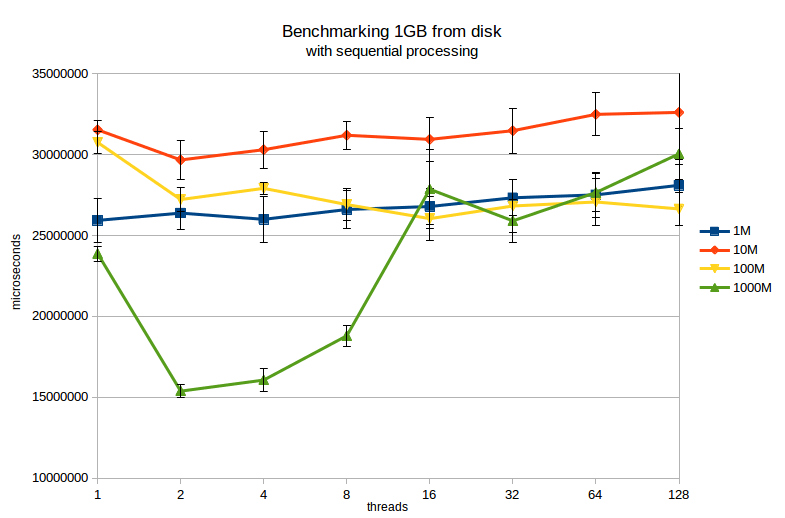
\includegraphics[scale=0.7]{../test_results/disk_seq.png}
  	\caption{These are the results from running the benchmarking method on a 1GB data from a file stream, with varying amounts of available memory, from 1 megabyte to 1 gigabyte. Processing of the data was done sequentially. The standard deviation resembles the standard deviation from the disk-benchmarking and lies from 1\% to 8\%.}
	\label{figure:disk-seq}
	\end{adjustwidth}
\end{figure}


\subsubsection{From memory}
The results from running the framework on streams of data that are already loaded into memory can be seen in \autoref{figure:mem-par} and in \autoref{figure:mem-seq}. The first one shows the results from running the system with parallel processing, where the second exhibits sequential processing. This is the ideal case, where we have a fast input stream, and we have a somewhat large amount of processing power available.\\

The practical timings in \autoref{table:io-test} shows that copying 1GB of memory takes approximately 0.2 seconds, this will be done twice in the benchmarking. First, when copying data to the worker buffers, and then to the output buffer. Further, the processing itself takes around 4.8 seconds. In total, that sums up to 5.2 seconds, if it were to be done sequentially.\\

The results shows that when we can perform sequential processing, the buffer-size does not make much of a difference. \autoref{figure:mem-par} clearly has very identical results for all four sizes of memory. With sequential processing, however, using the most memory clearly makes the framework faster. Larger buffers results in more processing, before switching threads, which in turn results in less overall locking and unlocking. The sequential processing manages to perform the benchmarks in approximately 4.8 seconds. This shows that the I/O has been hidden completely, and only the processing itself takes time. The parallel processing performs the benchmarking in approximately 1.6 seconds, effectively making it approximately 3.5 times faster thant the sequential processing. There is some inherent overhead from multithreading, which is why we can't achieve a 4 times speed-up with 4 cores.\\

The results also shows that with 1 thread, the timings match with performing the calculations in sequence. \autoref{figure:mem-seq} shows that with smaller amounts of memory, the locking becomes more expensive, with multiple threads. With 1M memory and 16 threads, there is a speed-up from 8 threads. The same tendency can be seen with 10M from 64 threads to 128 threads. This behaviour is hard to explain, and I have no apparent explanation. However, with plenty of memory, the sequential system performs best at around 8 threads. 


% Memory Parallel
\begin{figure}
	\begin{adjustwidth}{-0.5in}{-0.5in}
    \centering
     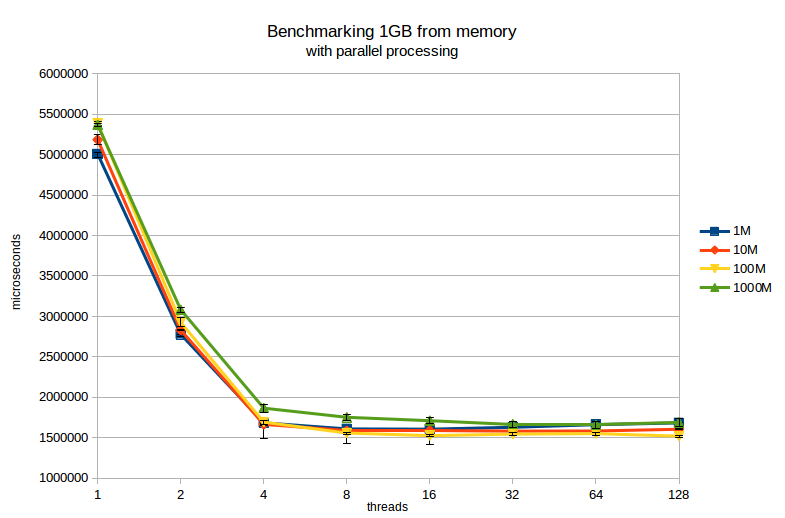
\includegraphics[scale=0.7]{../test_results/mem_par.png}
  	\caption{These are the results from running the benchmarking method on a 1GB data from main memory, with varying amounts of available memory, from 1 megabyte to 1 gigabyte. Processing of the data was done in parallel. The standard deviation resembles the standard deviation from the memory-benchmarking and lies from 1\% to 2\%.}
	\label{figure:mem-par}
	\end{adjustwidth}
\end{figure}

% Memory Sequential
\begin{figure}
	\begin{adjustwidth}{-0.5in}{-0.5in}
    \centering
     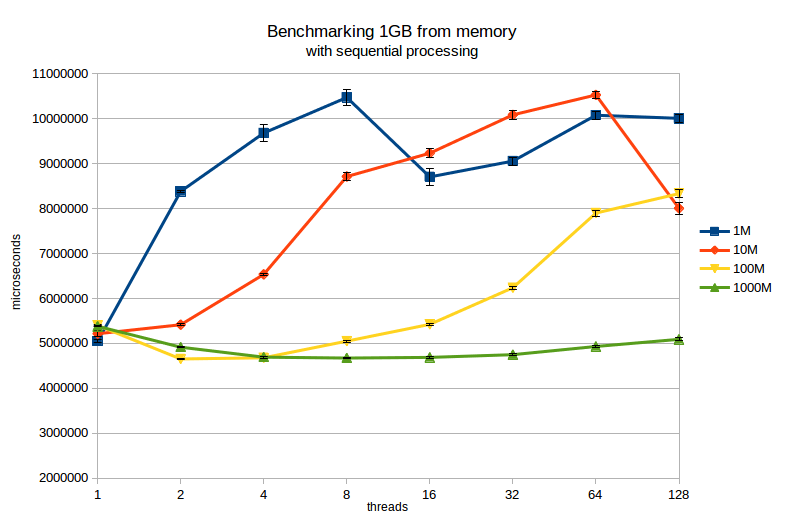
\includegraphics[scale=0.7]{../test_results/mem_seq.png}
  	\caption{These are the results from running the benchmarking method on a 1GB data from main memory, with varying amounts of available memory, from 1 megabyte to 1 gigabyte. Processing of the data was done sequentially. standard deviation resembles the standard deviation from the memory-benchmarking and lies from 1\% to 2\%.}
	\label{figure:mem-seq}
	\end{adjustwidth}
\end{figure}


\newpage
\section{Conclusion}
The \nbuf framework has been built with one main purpose. It should allow users with less experience in writing multithreaded applications to perform optimal and parallel I/O. This entails two different criteria. 

The first criteria depends on whether the framework really exhibits optimal I/O. The second criteria depends on whether the task of abstracting away the concurrency has created an interface that requires less multithreading experience to use.


\subsection{Performance}
Benchmarking the \nbuf framework has been done with a method that finds minimum and maximum values, and calculates an average value. This is a very light computation, and as such leaves most of the execution time of the framework to performing I/O. This is a good thing, because it lets us see directly, how the speed of the I/O resources affects the performance of the framework.\\

When working with a slow stream, the framework benefits from having a large amount of memory. Further, having more threads than there are hardware threads for, only reduces the efficiency. 

When using a slow hard disk drive, the sequential operation takes approximately 18.2 seconds, where the optimal configuration of the framework only takes approximately 15.1 seconds. The practical limit is approximately 13.4 seconds. This is independent of whether we perform sequential or parallel execution.\\

When working with a fast stream, the framework exhibits different behaviours when performing parallel processing and sequential processing. With sequential processing, having a large amount of memory helps. With parallel processing, the amount of memory doesn't make a large difference. In both cases, the optimal amount of threads matches with the amount of hardware threads. 

The the benchmarking task can be done sequentially in approximately 5.2 seconds, and the framework performs the benchmarking task in approximately 1.6 seconds. This is a factor 3.5 speed-up, which aligns with the 4 hardware cores on the system at hand.\\

To sum up, both with slow and fast I/O streams, speed-ups were achieved as expected. The highest throughput was obtained when having a fast stream, and parallel processing. When working with a slow stream, allocating extra memory gives a higher throughput. Using more threads than the hardware supports never gives higher throughput.


\subsection{Usefulness}
Producing on the \nbuf framework has resulted in a C++11 library that can be included by people with less experience with multi threaded applications. The library has been proven to increase performance whenever data is too large to fit in main memory, or when a small memory footprint is desired and larger amounts of data needs to be processed.

The framework gives access to native threading on most *NIX, while exposing an interface where no locks or synchronization has to be handled. The user of the library still has to know to what extend he can parallelize the task at hand, so that the task is solved correctly. This does require some amount of knowledge about how concurrency works.\\

Concurrency is inherently hard, and the framework performs correct concurrency. Users who decide to include this library will be able to perform tasks with efficient and parallel I/O, without having to debug for race conditions. This was the intention, and the framework solves the problem.\\

The framework does not yet support the queue mechanics, which is necessary for computational tasks which require more synchronization. This limitation decreases the usefulness of the system. Implementing such queue mechanic can be done rather easily, and therefore this is \textit{not a big problem}. The design has already been laid out.\\

The \nbuf framework is already available for people to work with through GitHub\footnote{The library is available on http://github.com/ath88/nbuf.}, and I expect to submit it to Boost\footnote{Boost is a repository for peer-reviewed C++ libraries. It can be found at http://www.boost.org.} if the code reaches maturity levels beyond this master's thesis.


\newpage
\section{Future Work}
\subsubsection{IO throttling}
not reading 1gb of data as a start, but starting low, and slowly increasing the buffer sizes.

\subsubsection{Variable buffer sizes}
When reading small files, allocating large buffers is unnecessary.

\subsubsection{Slow network? How does istream handle that}





\bibliographystyle{abbrv}
\bibliography{bib}





\end{document}